\documentclass[12pt,onecolumn]{article}

\usepackage{listings}
\usepackage{float}
\usepackage{mathtools}
\usepackage[russian]{babel}
\everymath{\displaystyle}

\usepackage[usenames]{color}
\usepackage{colortbl}

\usepackage{geometry}
\usepackage{minted}
\geometry{
  a4paper,
  top=15mm, 
  right=10mm, 
  bottom=15mm, 
  left=10mm
}

\definecolor{dkgreen}{rgb}{0,0.6,0}
\definecolor{gray}{rgb}{0.5,0.5,0.5}
\definecolor{mauve}{rgb}{0.58,0,0.82}

\lstset{frame=tb,
  language=sh,
    aboveskip=3mm,
      belowskip=3mm,
        showstringspaces=false,
	  columns=flexible,
	    basicstyle={\small\ttfamily},
	      numbers=none,
	        numberstyle=\tiny\color{gray},
		  keywordstyle=\color{blue},
		    commentstyle=\color{dkgreen},
		      stringstyle=\color{mauve},
		        breaklines=true,
			  breakatwhitespace=true,
			    tabsize=3
			    }
\begin{document}

\begin{center}
    Федеральное государственное автономное образовательное учреждение высшего образования\\
	«Национальный исследовательский университет ИТМО»
\end{center}
\vspace{1cm}
\setcounter{page}{0} 
\begin{center}
    \large \textbf{Отчет}\\
    \textbf{по лабораторной работе №2}\\
    \large \textbf{«Синтез помехоустойчивого кода»}\\
     по дисциплине «Информатика»\\
	\vspace{1cm}
    Вариант №79\\
\end{center}

\vspace{10cm}
\begin{flushright}
  Выполнил: Кокорин Всеволод Вячеславович, группа P3118\\
  Преподаватель: Рыбаков Степан Дмитриевич\\
\end{flushright}

\vspace{5cm}
\begin{center}
    г. Санкт-Петербург\\
    2022г.
\end{center}
\thispagestyle{empty}
\newpage
\tableofcontents
\newpage
\section{Схема декодирования классического кода Хэмминга (7;4)}
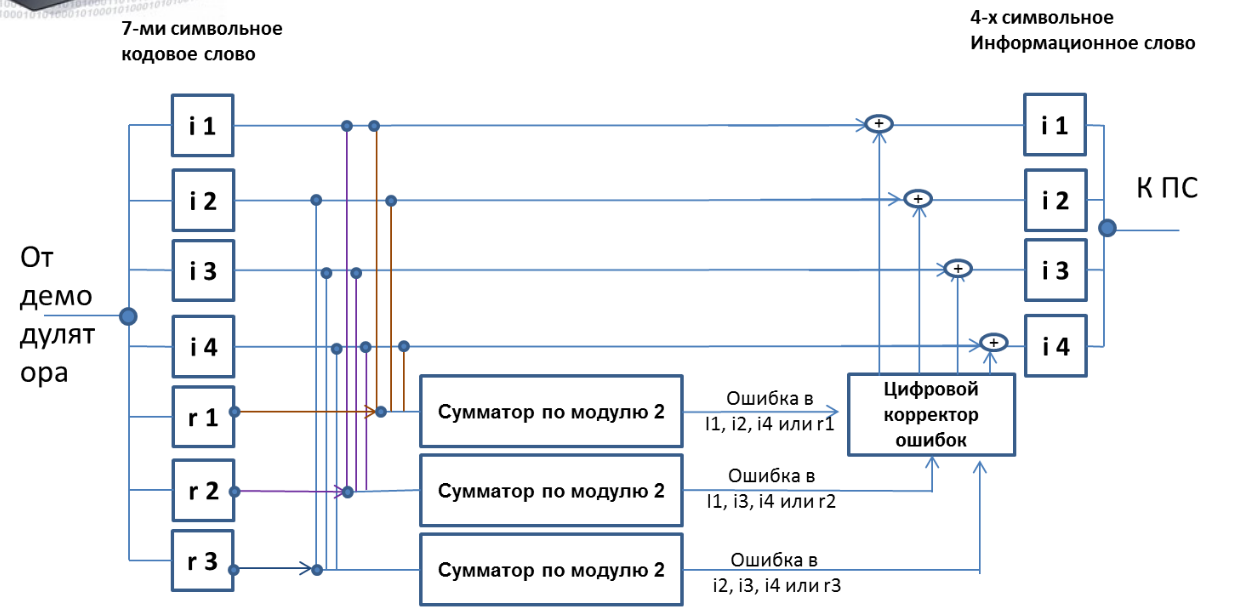
\includegraphics[width=15cm]{img/img1.png}
\newpage
\section{1 задача}
1. (63)  0110100 \\
   Синдром:\\
   $S_1$ = (0 + 1 + 1 + 0) \% 2 = 0\\
   $S_2$ = (1 + 1 + 0 + 0) \% 2 = 0\\
   $S_3$ = (0 + 1 + 0 + 0) \% 2 = 1\\
   4 бит передан неправильно. \\
   1100 - переданное сообщение. \\ 
\\
\\
2. (10) 1010000 \\
   Синдром: \\
   1. $S_1$ = (1 + 1 + 0 + 0) \% 2 = 0\\
   2. $S_2$ = (0 + 1 + 0 + 0) \% 2 = 1\\
   4. $S_3$ = (0 + 0 + 0 + 0) \% 2 = 0\\
   2 бит переданн неправильно. \\
   1000 - переданное сообщение. \\
\\
\\
3. (35) 0111010 \\
   Синдром: \\
   1. $S_1$ = (0 + 1 + 0 + 0) \% 2 = 1\\
   2. $S_2$ = (1 + 1 + 1 + 0) \% 2 = 1\\ 
   4. $S_3$ = (1 + 0 + 1 + 0) \% 2 = 0\\ 
   3 бит переданн неверно.
   0010 - переданное сообщение. \\
\\
\\
4. (75) 0101101 \\
   Синдром: \\
   1. $S_1$ = (0 + 0 + 1 + 1) \% 2 = 0 \\
   2. $S_2$ = (1 + 0 + 0 + 1) \% 2 = 0\\
   4. $S_3$ = (1 + 1 + 0 + 1) \% 2 = 1\\
   4 бит передан неправильно. \\
   0101 - переданное сообщение. \\
\newpage
\section{Схема декодирования классического кода Хэмминга (15;11)}
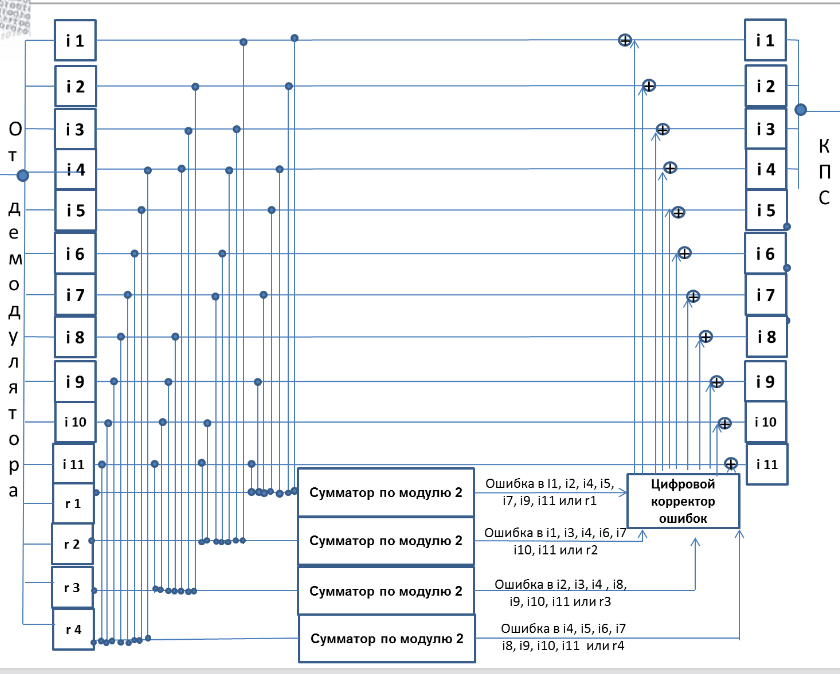
\includegraphics[width=15cm]{img/img2.png}
\newpage
\section{2 задача}
(78) 001110010110100 \\
   Синдром:\\
   1. $S_1$ = (0 + 1 + 1 + 0 + 0 + 1 + 1 + 0) \% 2 = 0\\
   2. $S_2$ = (0 + 1 + 0 + 0 + 1 + 1 + 0 + 0) \% 2 = 1\\
   4. $S_3$ = (1 + 1 + 0 + 0 + 1 + 0 + 0 + 0) \% 2 = 1\\
   8. $S_4$ = (1 + 0 + 1 + 1 + 0 + 1 + 0 + 0) \% 2 = 0\\
   6 бит передан неправильно.\\
   11100110100 - переданное сообщение.
\newpage
\section{3 задача}
  i = (63 + 10 + 35 + 75 + 78) * 4 = 1044\\
  \\
  $2^r$ - r - 1 = 1044\\
  \\
  r \approx 10.043086 ,r \in \mathbb{N} \Rightarrow r  = 11\\
  \\
  Ans = $$\frac{r}{i + r}$$ = \frac{11}{1055} \approx 0.01042654028436019\\
  \\
\newpage
\section{Вывод}
По ходу выполнения данной работы, я узнал про помехоустойчивые коды, научился кодировать и декодировать сообщения с помощью кода Хэмминга.
\newpage
\section{Список литературы}
"Код Хэмминга. Пример работы алгоритма" \textbf{[Электронный ресурс].} - Текст: электронный // habr.com – URL: https://habr.com/ru/post/140611/ \\
"Помехоустойчивое кодирование с иcпользованием различных кодов" \textbf{[Электронный ресурс].} - Текст: электронный // habr.com – URL: https://habr.com/ru/post/111336/ \\
"Помехоустойчивое кодирование. Часть 1: код Хэмминга" \textbf{[Электронный ресурс].} - Текст: электронный // habr.com – URL: https://habr.com/ru/post/357666/
\end{document}
